The following sections aim to describe the integration testing sequence of the different components and subsystems of \emph{PowerEnJoy}. From now on the following notation will be used: C1 $\rightarrow$ C2 indicates that C2 is necessary for C1 to work properly.

\subsection{Software Integration Sequence}
The components of each subsystem are tested starting from the most to the least independent one.

\subsubsection{Data Access}
%DBMS <- JEBs
The first components to be integrated are those relative to the data access, starting from the database core: the DBMS. This will be integrated with all the Java Entity Beans (JEB) defined in the Design Document~\cite{dd}. 

%---------------------ATTENZIONE------------------------------
%definiamole però!
%Secondo me possiamo unificare i due passaggi. Partiamo dalle entity beans che hanno bisogno di driver per verificare che i loro metodi, opportunamente invocati, producano query corrette. Inutile il passaggio intermedio di creare driver rappresentanti le singole JEB. Perchè poi?

In order to do so, the DBMS will need a driver for each Entity Bean to carry out queries and verify their correctness on a dummy database, containing a greatly reduced number of test information. Said test database will be structured based on the E-R schema that will be adopted for the final implementation of the data layer.

%----- PEZZO CAMBIATO -------
%In order to do so, the DBMS will need a driver for each Entity Bean to simulate actual queries and their correctness on a dummy database, containing a greatly reduced number of test information. Said test database will be structured based on the E-R schema that will be adopted for the final implementation of the data layer.

\begin{figure}[H]
\begin{center}
		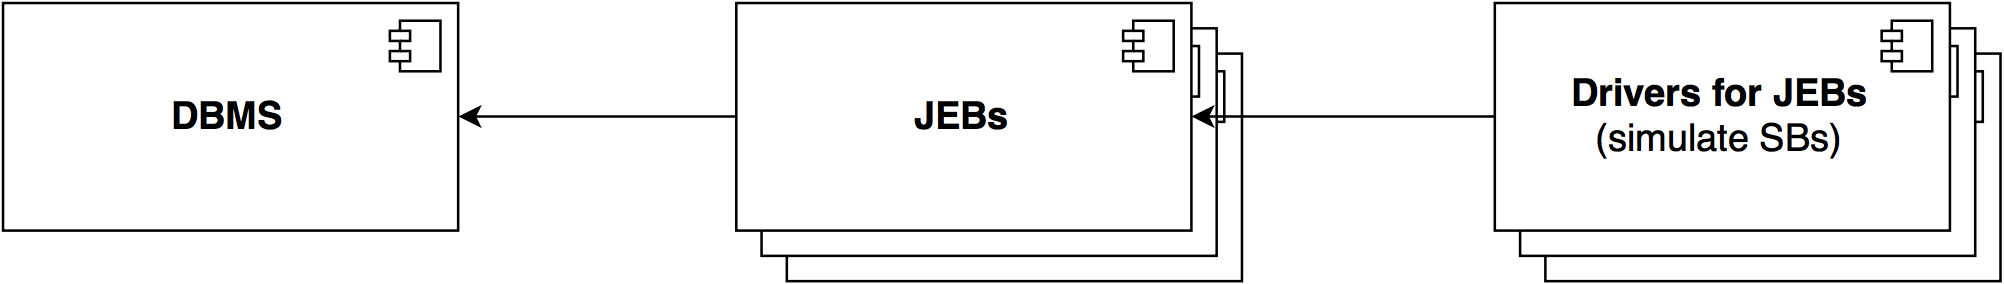
\includegraphics[width=\textwidth]{./integration_strategy/diagrams/data_access.png}
\end{center}
\end{figure}

%JEB User <- UserManager
%JEB User <- SecurityAuthenticator
%JEB Car <- CarStatusManager
%JEB Car <- ReservationManager
%JEB Car <- MapManager
%JEB Reservation <- ReservationManager
%JEB Reservation <- SecurityAuthenticator
%JEB Ride <- RideManager
%JEB SafeArea <- MapManager
%JEB PowerGridStation <- MapManager
%JEB AlternativeChargesSituation <- DiscountProvider
%JEB Payment <- PaymentGateway
\noindent
The next steps involve the integration of the Session Beans which take the advantage of said Entity Beans and are in charge of accessing them in the final application.

%----- PEZZO CAMBIATO -------
%The next steps involve the definition of the needed drivers for each of the JEB. These drivers represent the Session Beans that will be in charge of accessing the individual Entity Beans in the final application.

%diagrammi con tutti i collegamenti

\subsubsection{User and Utilities Management}
%NotificationManager <- UserManager
%NotificationManager <- PaymentGateway
%UserManager <- PaymentGateway
The integration can begin by covering the user management and the business logic utilities, that are considered relevant to support the rest of the application functionalities. To begin with, the most independent bean is, in this case, the NotificationManager, that requires drivers to invoke and test methods later used by UserManager and PaymentGateway (1).
\noindent
The UserManager component can then in turn be integrated (2), using the same driver used in the previous step to replace the PaymentGateway and to call the needed methods appropriately for the case.

\begin{figure}[H]
\begin{center}
		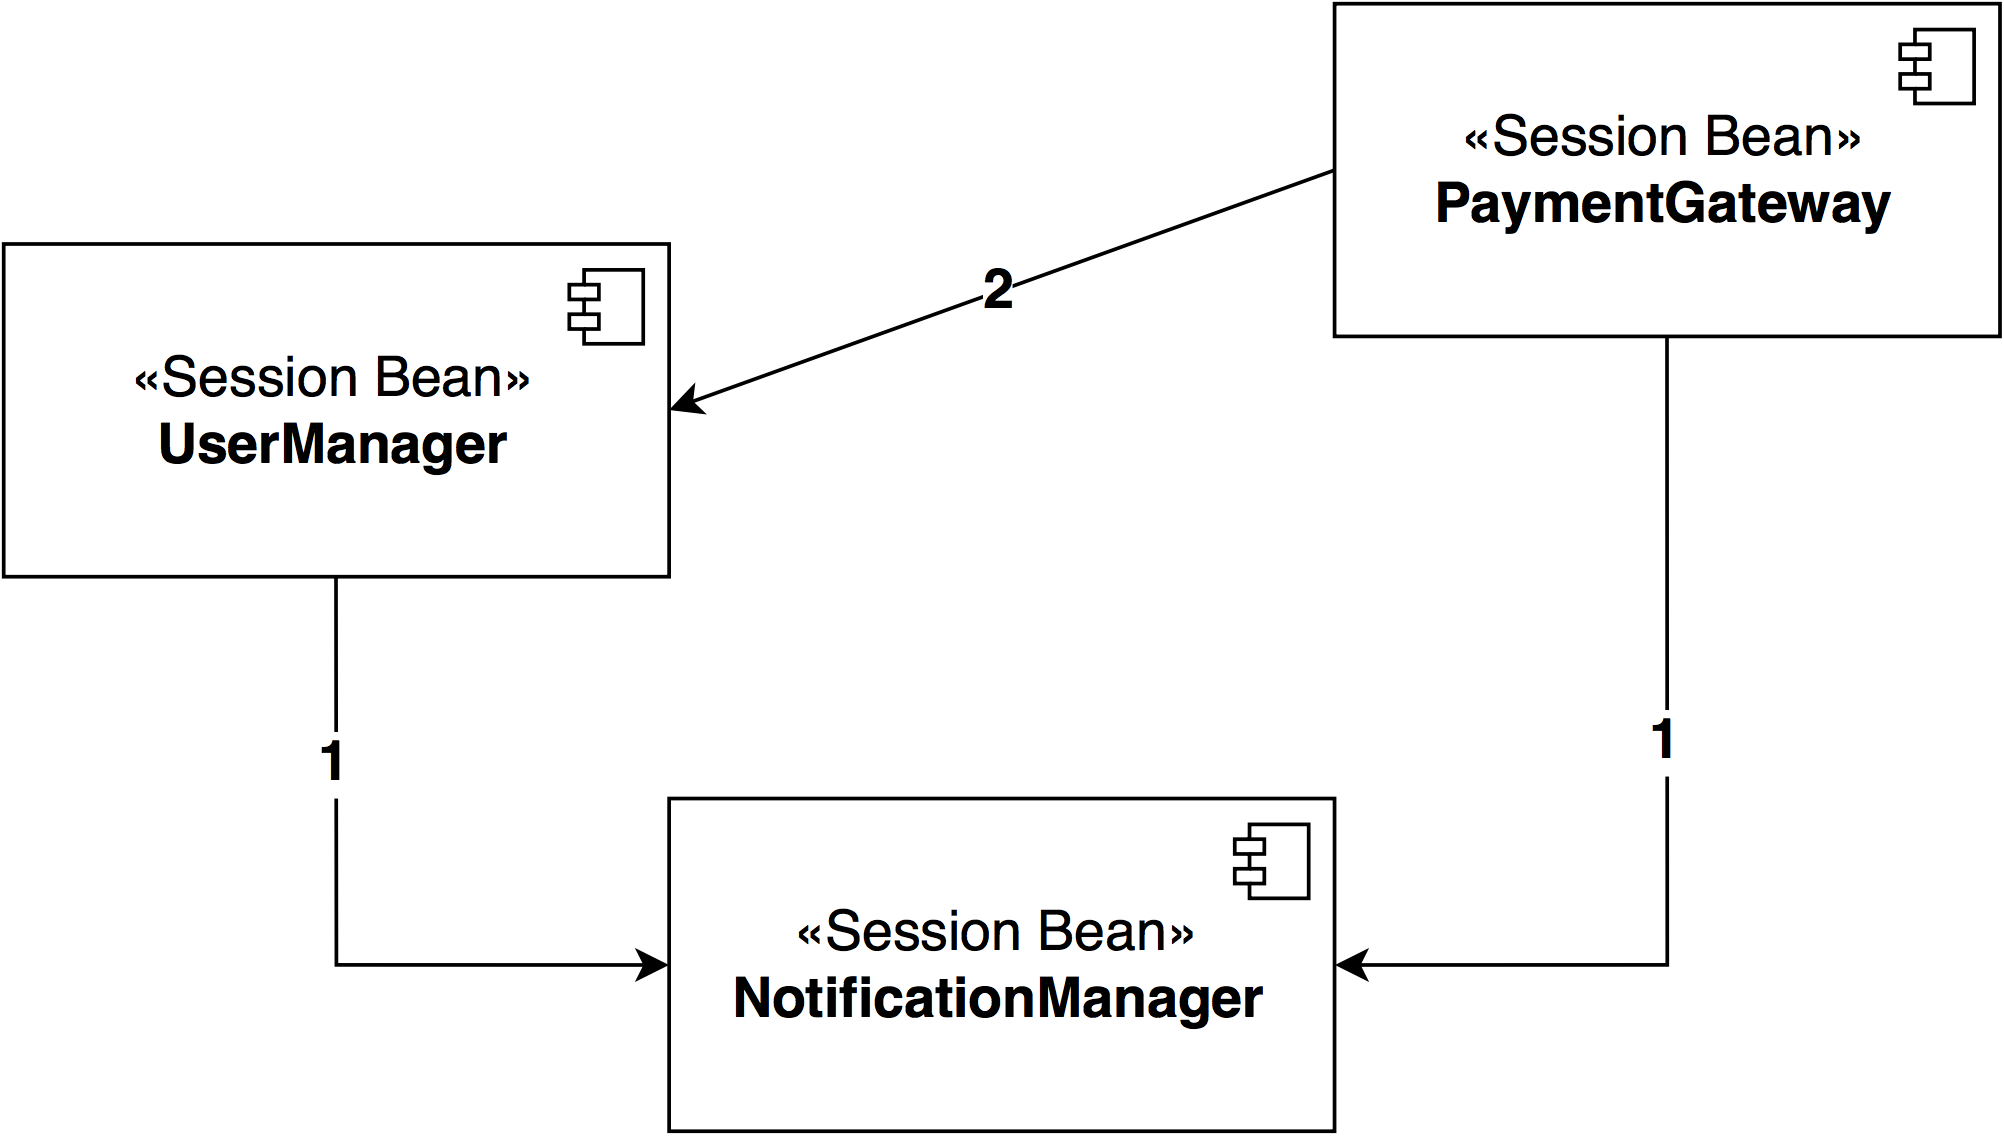
\includegraphics[width=0.8\textwidth]{./integration_strategy/diagrams/user_utilities.png}
\end{center}
\end{figure}

\subsubsection{Payment Management}
%DiscountProvider <- RideManager
%DiscountProvider <- PaymentGateway
%PaymentGateway <- RideManager
The payment management context can be covered next in the integration process, starting once more from the most independent component, represented by the DiscountProvider. This will need two different drivers, one for the methods called by the RideManager and another for the PaymentGateway (1).
\noindent
The PaymentGateway itself can in turn be integrated by using the same driver used before to replace the RideManager (2), only with the appropriate functionalities.

\begin{figure}[H]
\begin{center}
		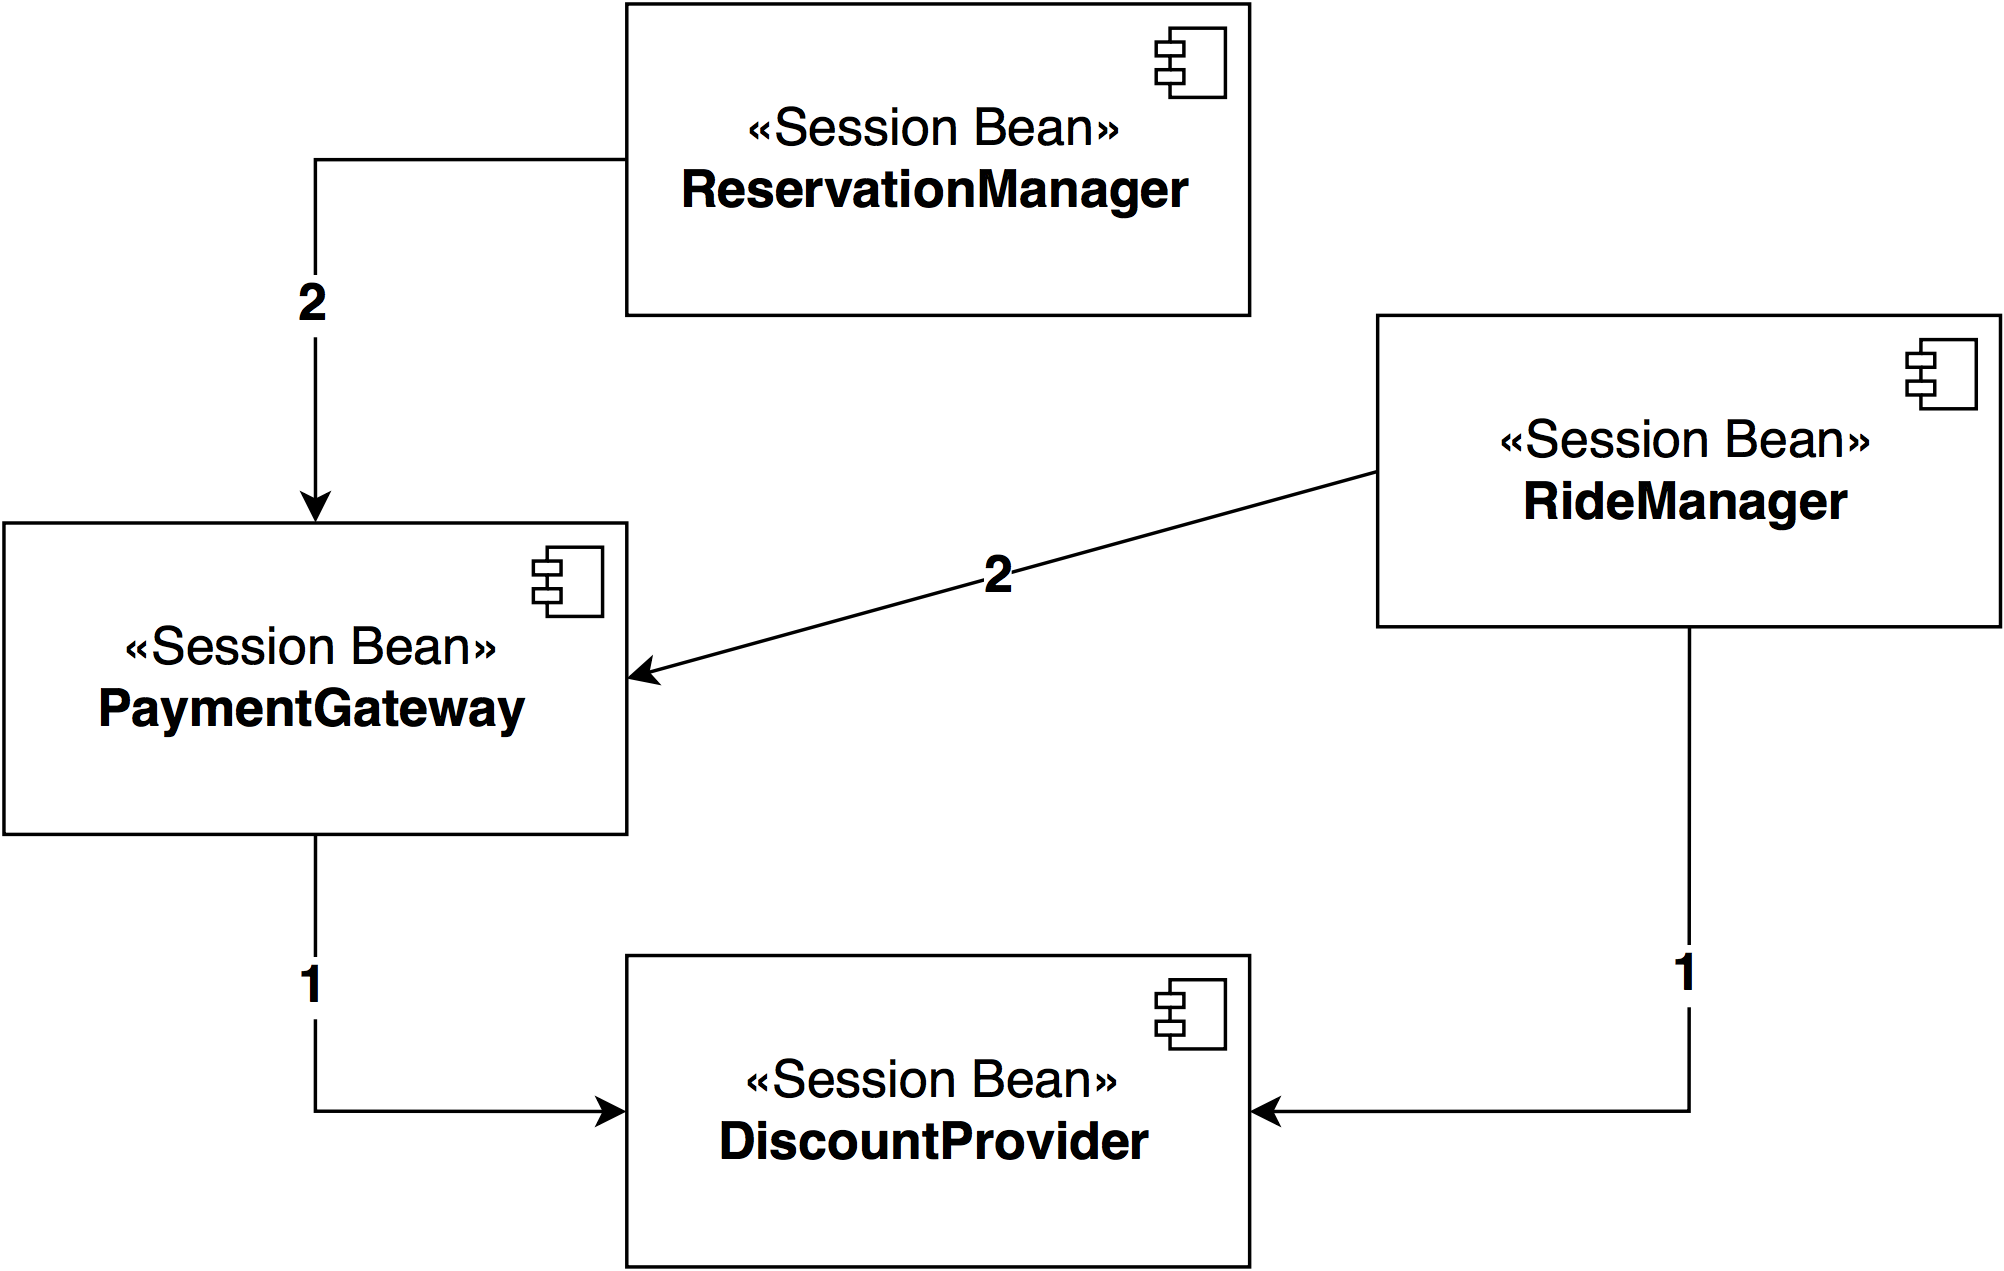
\includegraphics[width=0.8\textwidth]{./integration_strategy/diagrams/payment.png}
\end{center}
\end{figure}

%----CONTINUARE COME SOPRA?

\subsubsection{Ride and Reservation Management}
%CarStatusManager <- RideManager	
%CarStatusManager <- ReservationManager
%RideManager <- SecurityAuthenticator
%SecurityAuthenticator <- MapManager
The most critical features of the application revolve around the management of rides and reservations. Within this context, the most independent functionality is provided by the CarStatusManager bean, since no other bean depends on it apart from the already integrated Entity Beans. In order to integrate the CarStatusManager, there will be the need of two drivers: one for the ReservationManager and one for the RideManager (1).
\noindent
In its turn, the RideManager itself needs a driver in order to be integrated (2), which will represent the SecurityAuthenticator session bean.
\noindent
The last component to be integrated in this context is the SecurityAuthenticator, which will need a driver for the MapManager bean (3).

\begin{figure}[H]
\begin{center}
		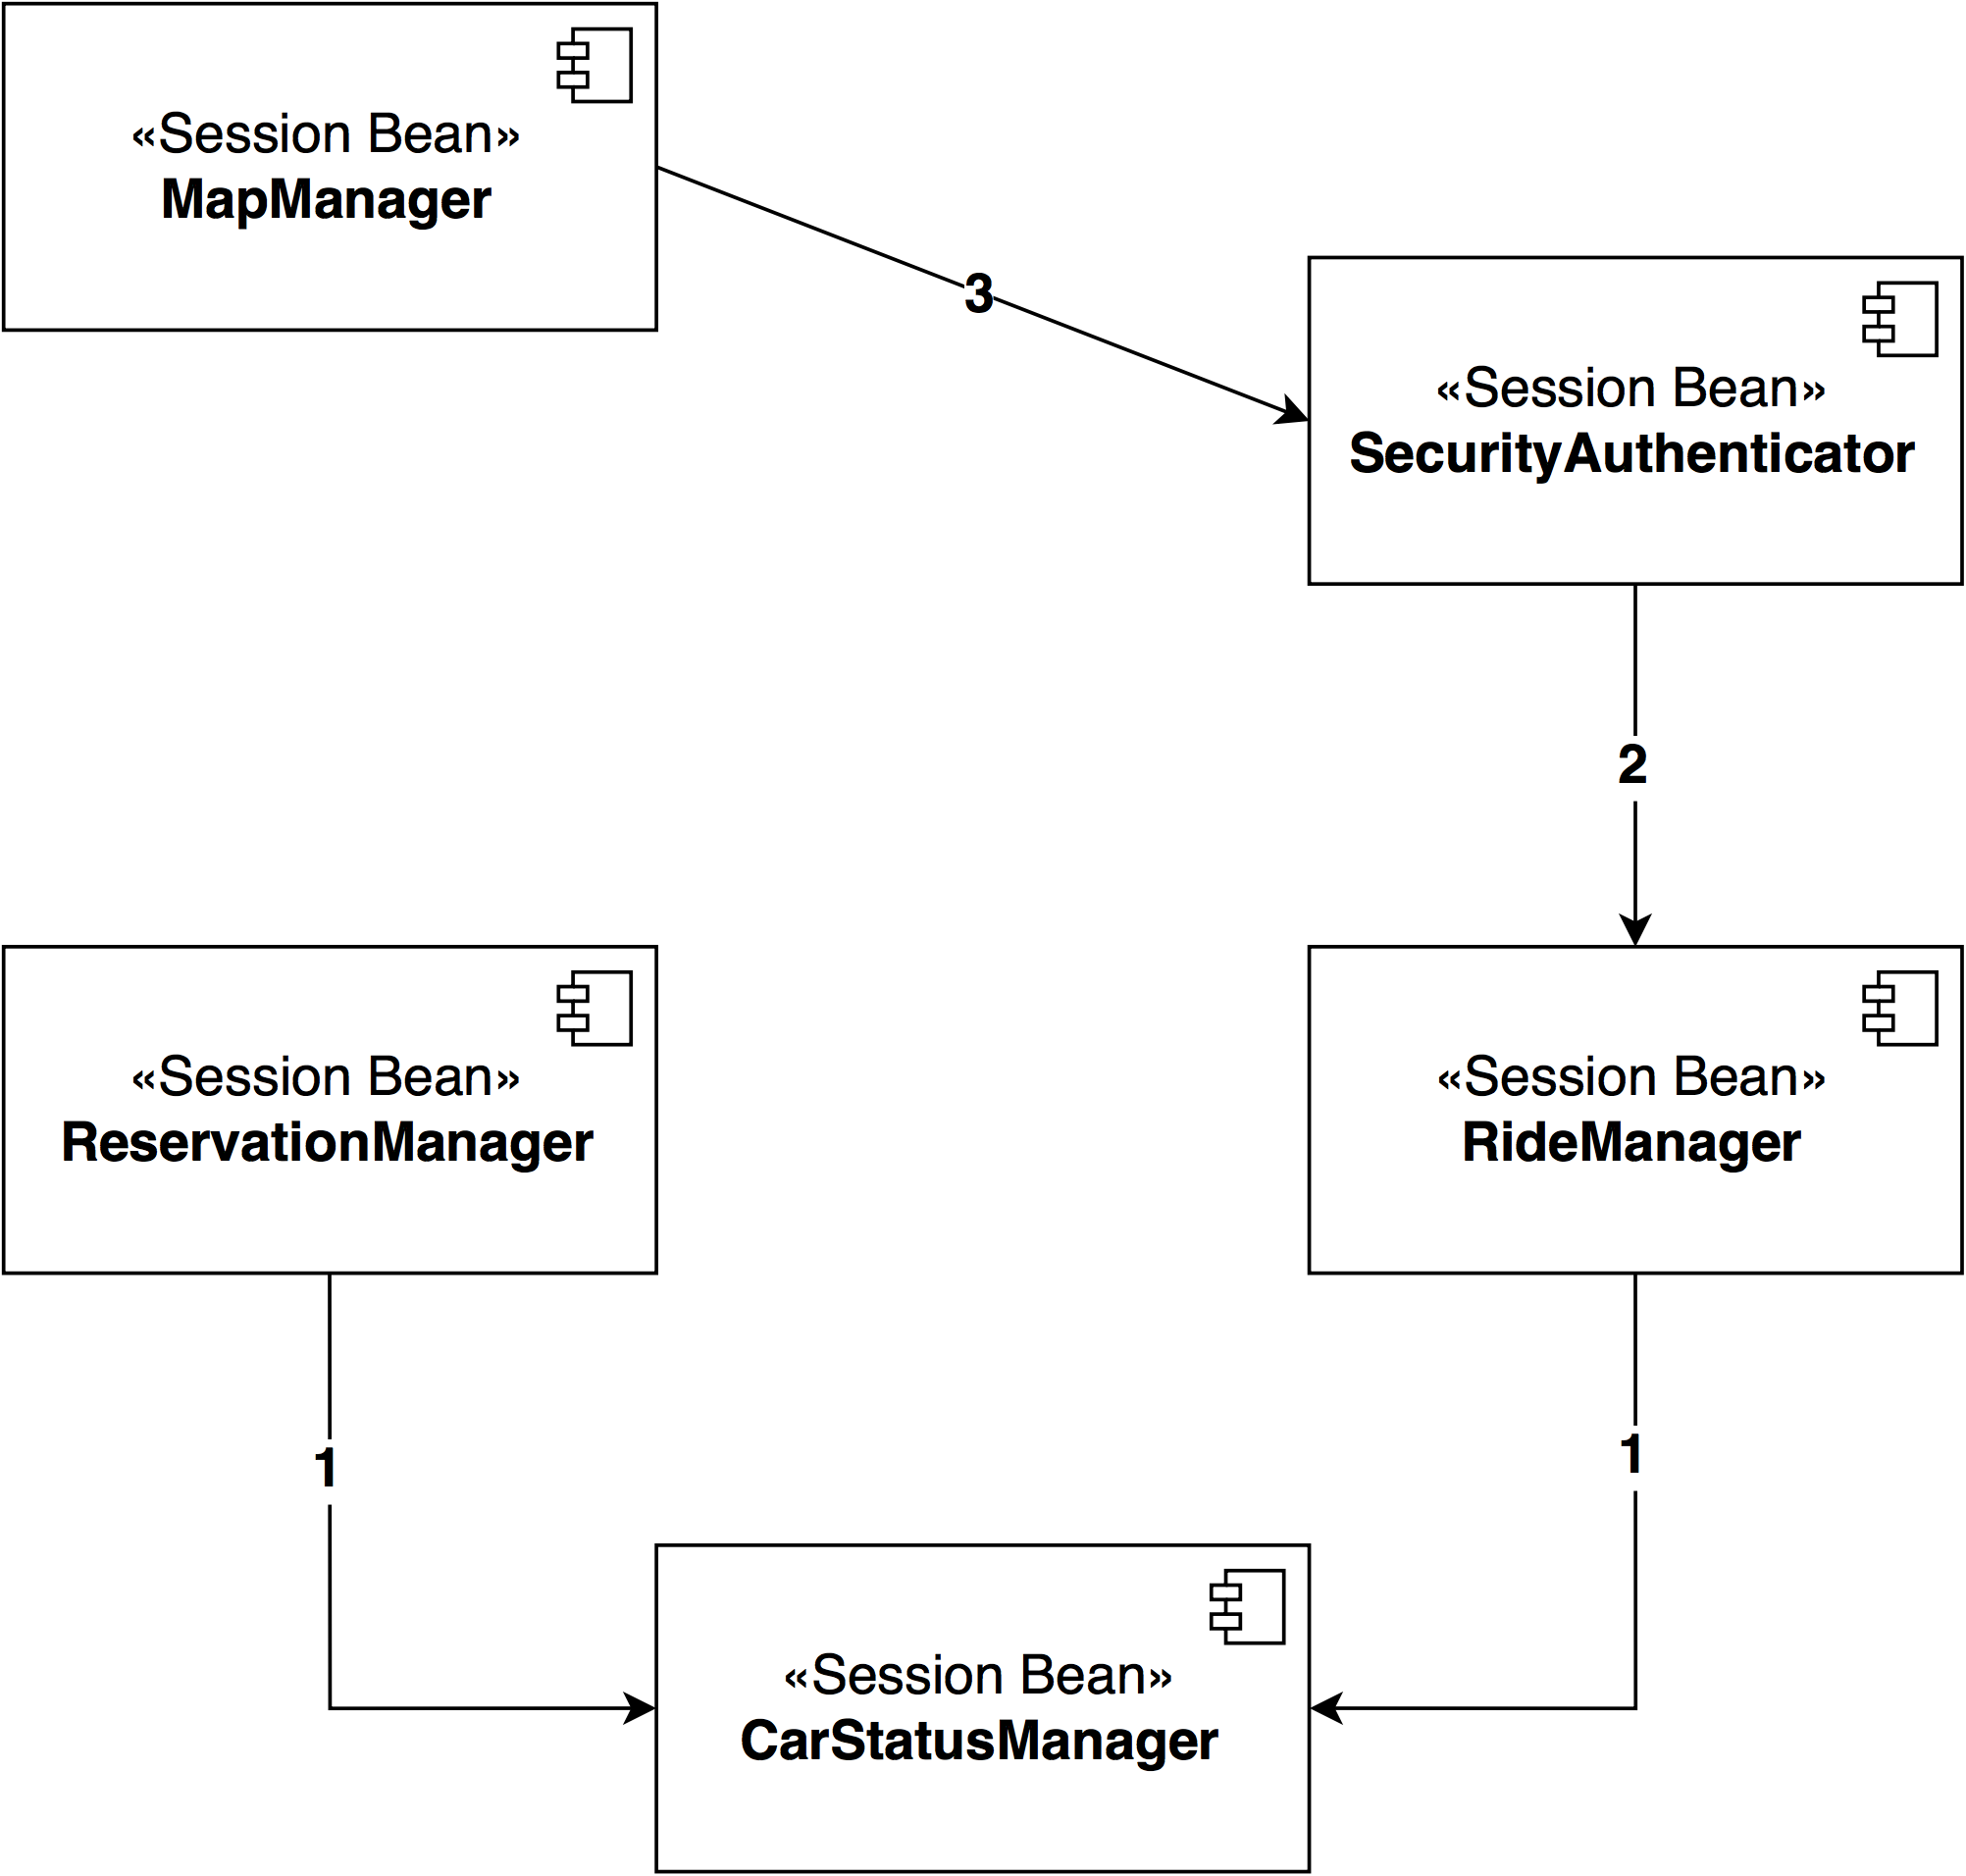
\includegraphics[width=0.8\textwidth]{./integration_strategy/diagrams/ride_reservation.png}
\end{center}
\end{figure}

\subsubsection{External Systems}
%STUB OF PAYMENT HANDLER ENDPOINT <- PaymentGateway
%CarStatusManager <- DRIVER FOR MAINTENANCE SYSTEM ENDPOINT
As stated in Section \ref{strategy} of this document, the relevance of the interactions with external systems makes it necessary to integrate some of said functionalities at an application logic level.
\noindent
To be precise, the components to be integrated are the endpoints of the Payment Handler and of the Maintenance System. Since in the final implementation of the application the Payment Handler will provide the APIs to interface with it, the integration will need a \emph{stub} of the Payment Handler endpoint, which will simulate the behaviour of the external payment system. The Maintenance System will instead use the APIs provided by the \textit{PowerEnJoy} system itself, hence the integration process will need a \emph{driver} for it.

\begin{figure}[H]
\begin{center}
		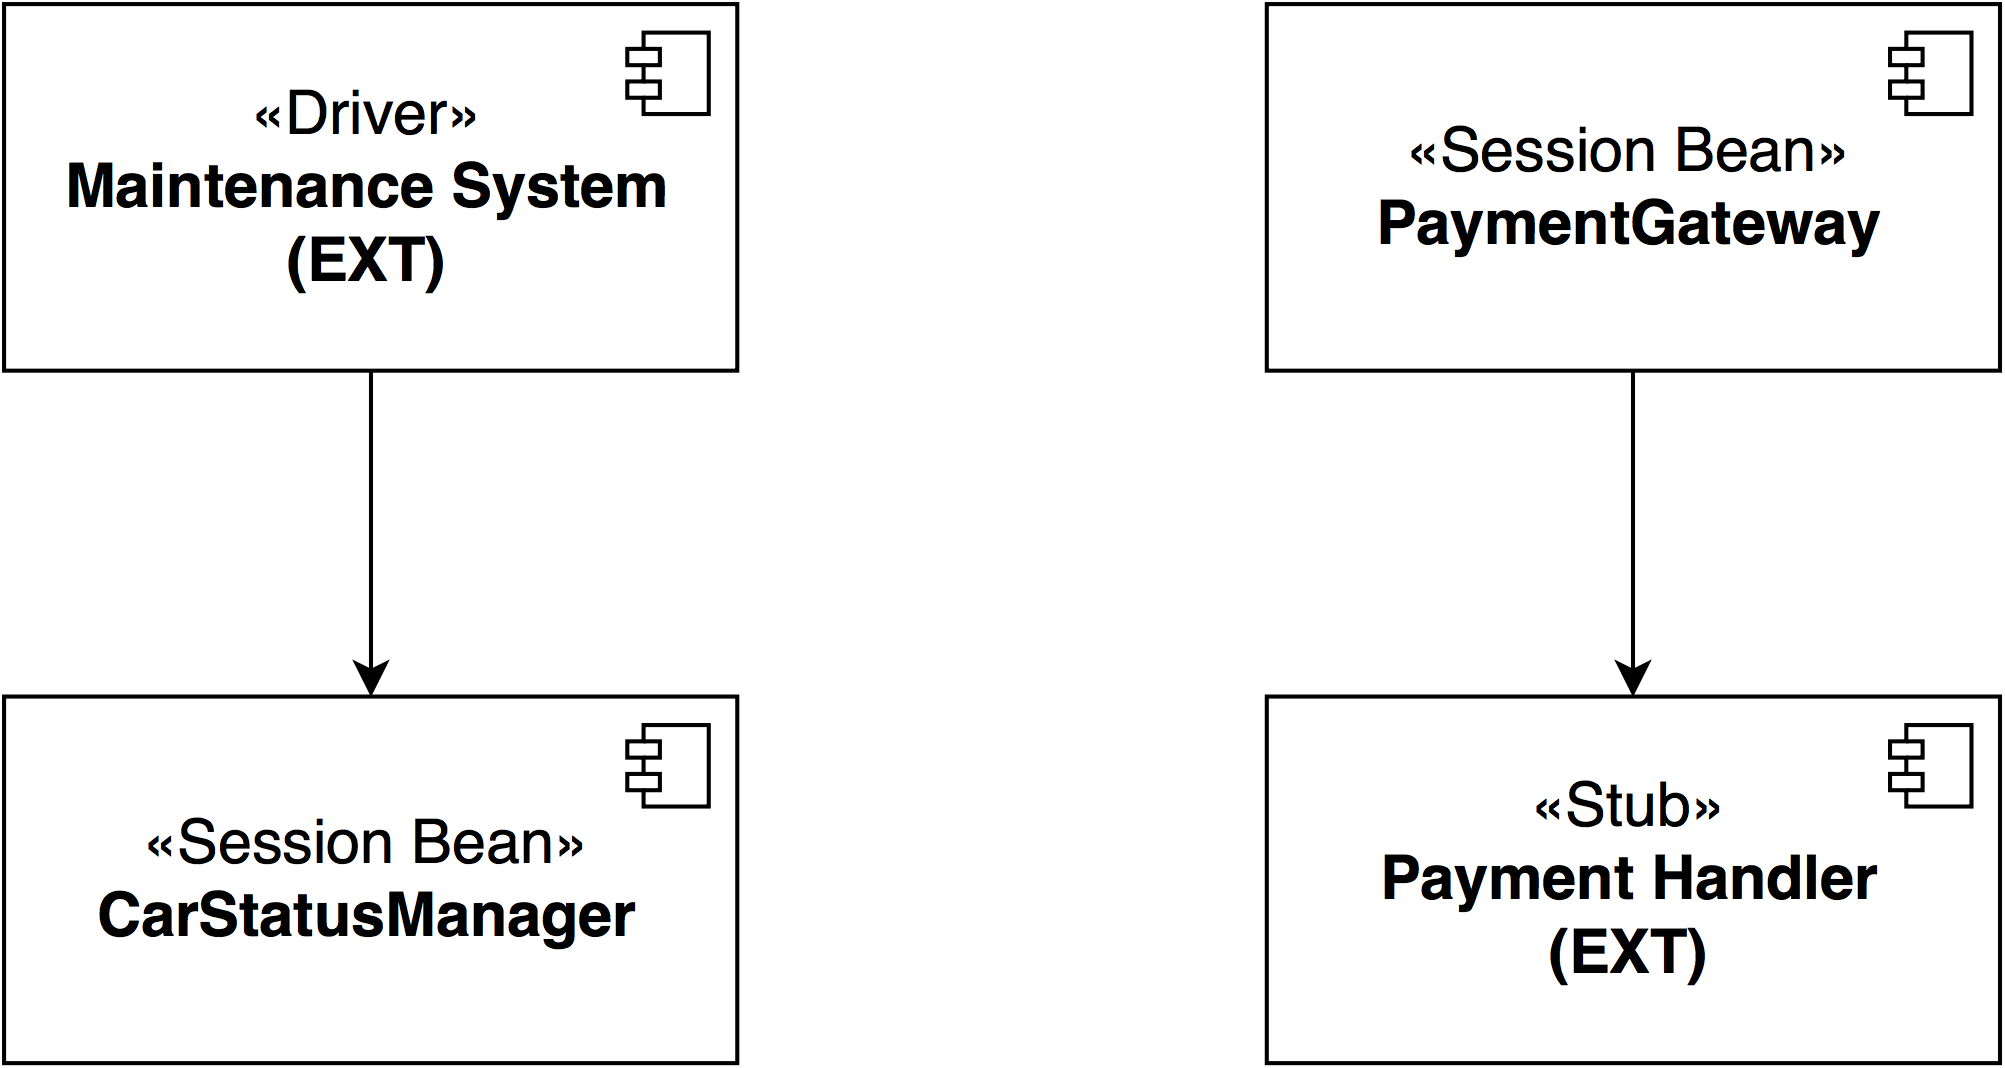
\includegraphics[width=0.8\textwidth]{./integration_strategy/diagrams/external_systems.png}
\end{center}
\end{figure}

\subsubsection{Application Logic Overall Integration}
%UserManager <- UserManagementContainer
%MapManager <- UtilitiesContainer
%NotificationManager <- UtilitiesContainer
%DiscountProvider <- ChargesManagementContainer
%PaymentGateway <- ChargesManagementContainer
%ReservationManager <- RideManagementContainer
%RideManager <- RideManagementContainer
%SecurityAuthenticator <- RideManagementContainer
%CarStatusManager <- RideManagementContainer
%ContainerController <- All containers
To conclude the integration process for the application logic tier, drivers for the EJB Containers must be provided, in order to have a means to simulate multiple requests for session bean instances; this will help in testing the underlying system effectiveness in managing heavy loads and concurrency during ordinary activity.
\noindent
Lastly, in order to simulate the correctness of requests to the individual containers, a driver for a ContainerController must be used to bypass the runtime behaviour and reproduce said requests in a deterministic way. This approach will avoid the necessity of implementing the whole system before having the possibility to test the correctness of the requests to the containers.
%DIAGRAMMONE GIGANTEEEE - didascalia: i numeri indicani i test case (livello software) in ordine di integrazione

\subsubsection{On-Board Application}
%GPSManager <- ApplicationController
%UIManager <- ApplicationController
%DataProcessingUnit <- ApplicationController
%ConnectivityUnit <- ApplicationController
The on-board application components integration will be affected by the central role of the application controller, for which a driver will be provided. This driver is going to serve its functions for every component of the application, since they all depend on it.

%---------------------ATTENZIONE------------------------------
%Rifrasare: il driver chiama tutti i metodi dei componenti a cui è collegato (non si capisce "serve its functions").

\begin{figure}[H]
\begin{center}
		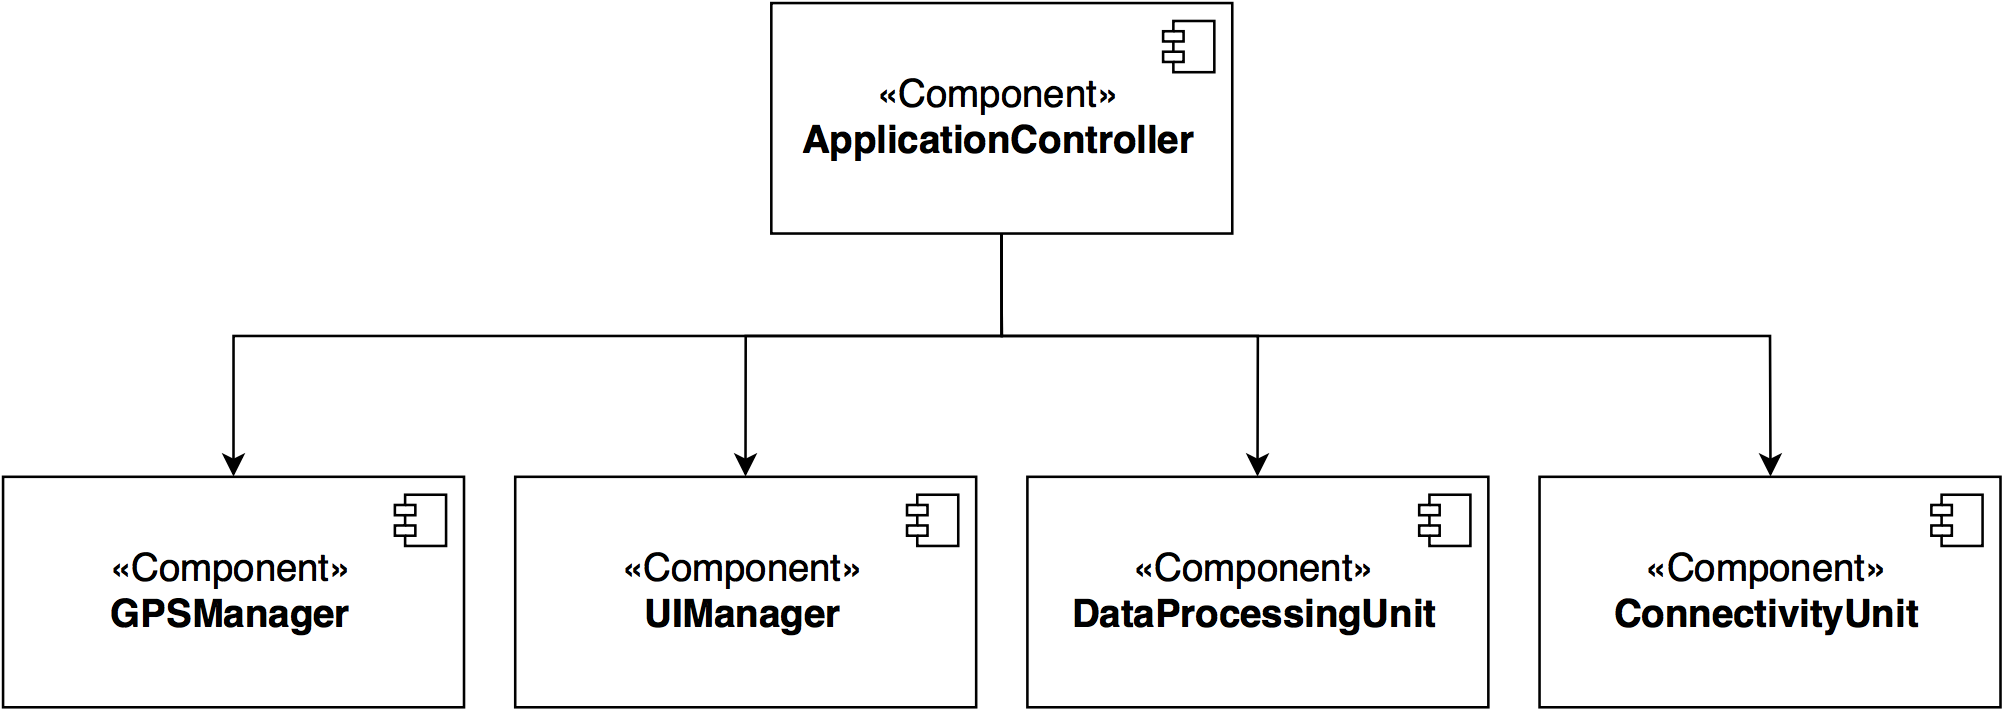
\includegraphics[width=\textwidth]{./integration_strategy/diagrams/on_board.png}
\end{center}
\end{figure}

\subsubsection{Mobile Application}
%GPSManager <- ApplicationController
%UIManager <- ApplicationController
Similarly to what is stated for the on-board application, the mobile application will follow the order imposed by the centrality of the application controller; the other components of the application will use a driver for the controller in order to be integrated.

\begin{figure}[H]
\begin{center}
		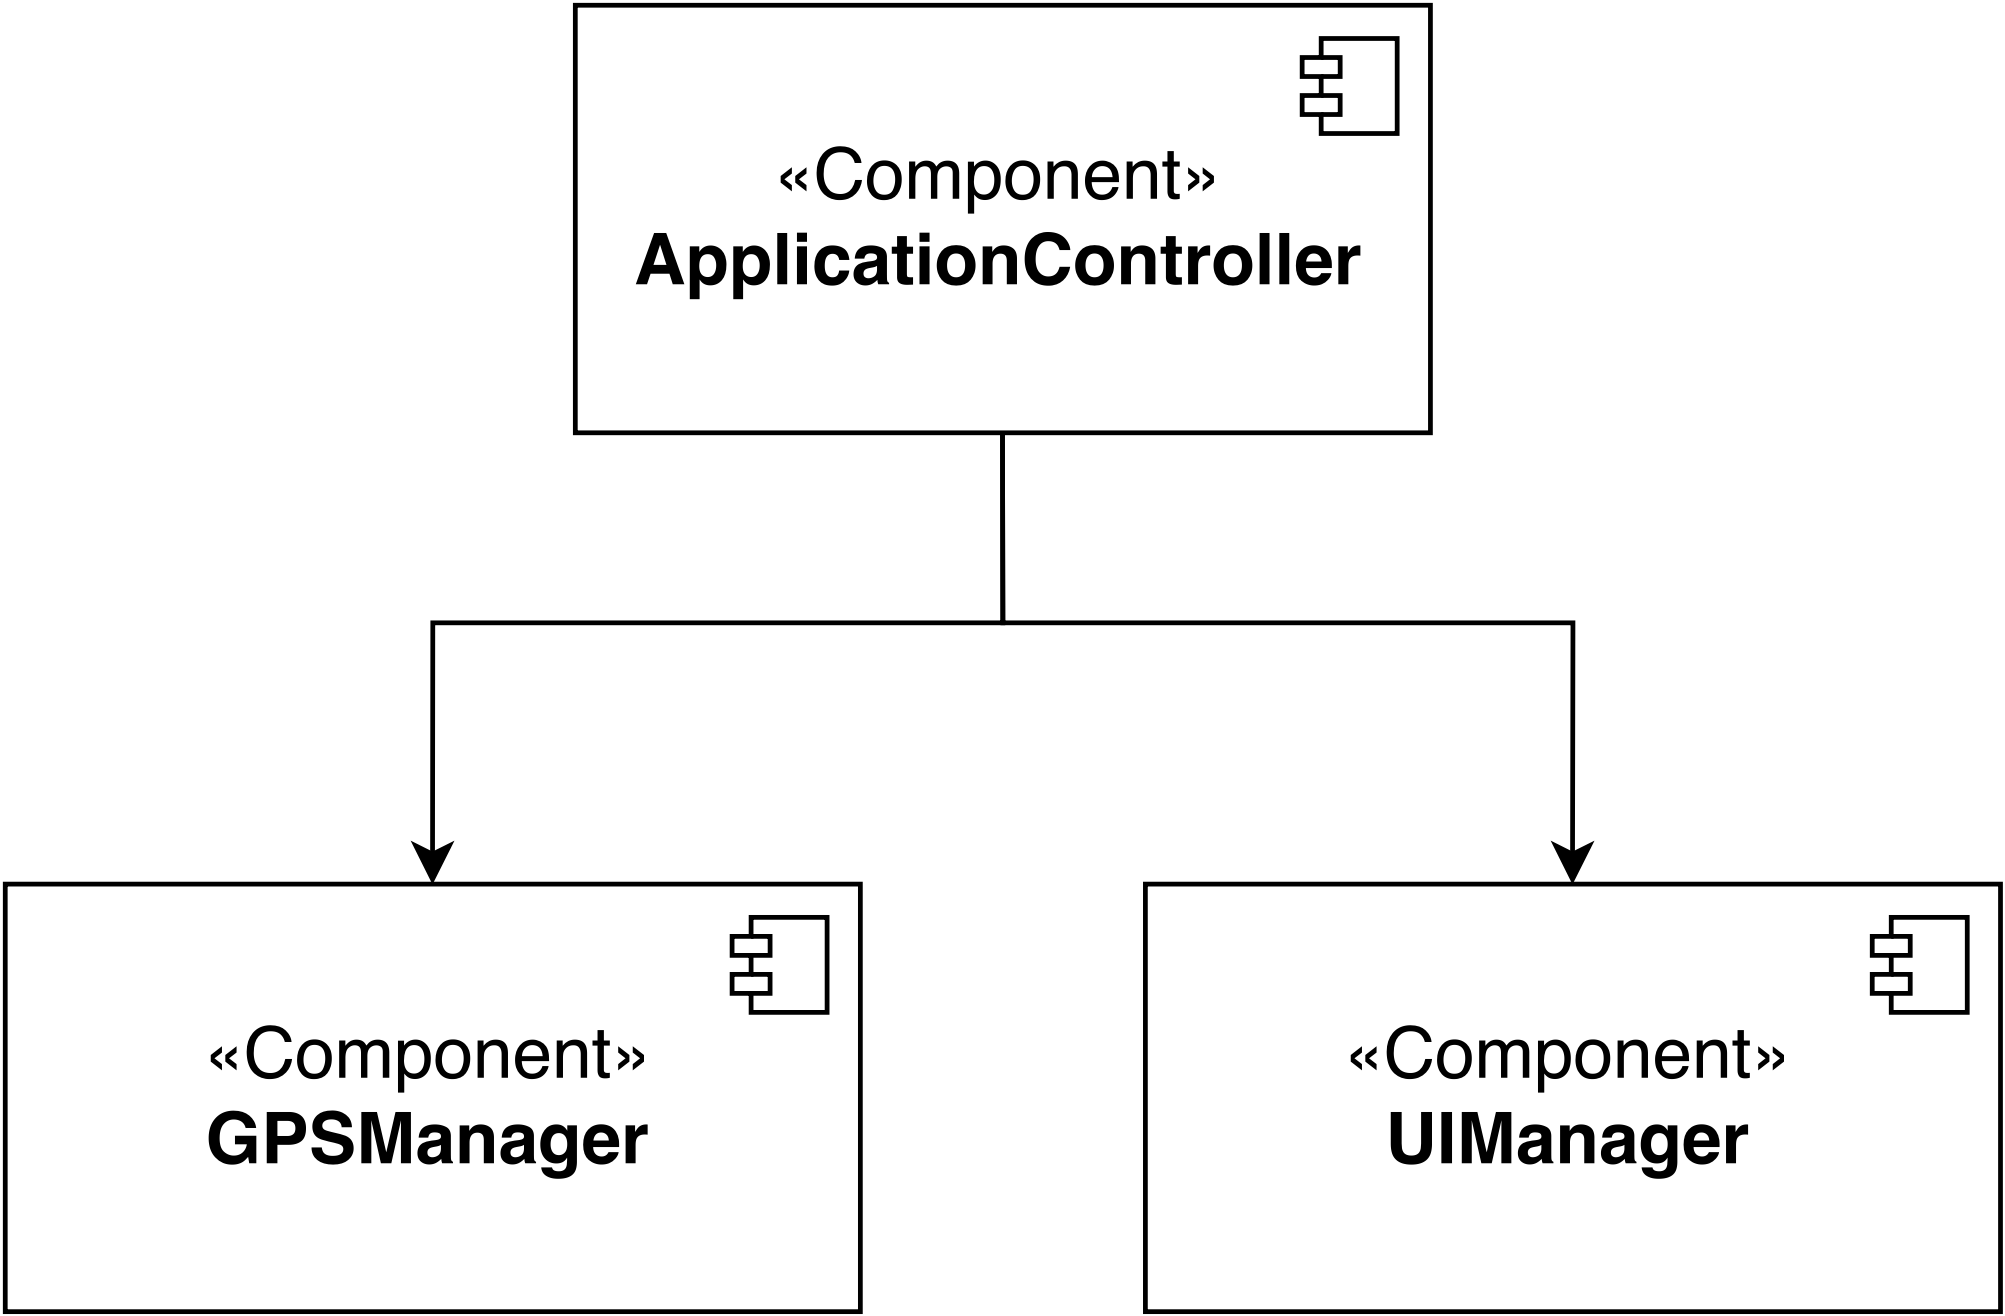
\includegraphics[width=0.6\textwidth]{./integration_strategy/diagrams/mobile.png}
\end{center}
\end{figure}

\subsubsection{Web Application}
%JavaServerPages <- WebController
The web application components will be integrated in a single step: a driver of the web controller will be used to integrate the JSP component.

\begin{figure}[H]
\begin{center}
		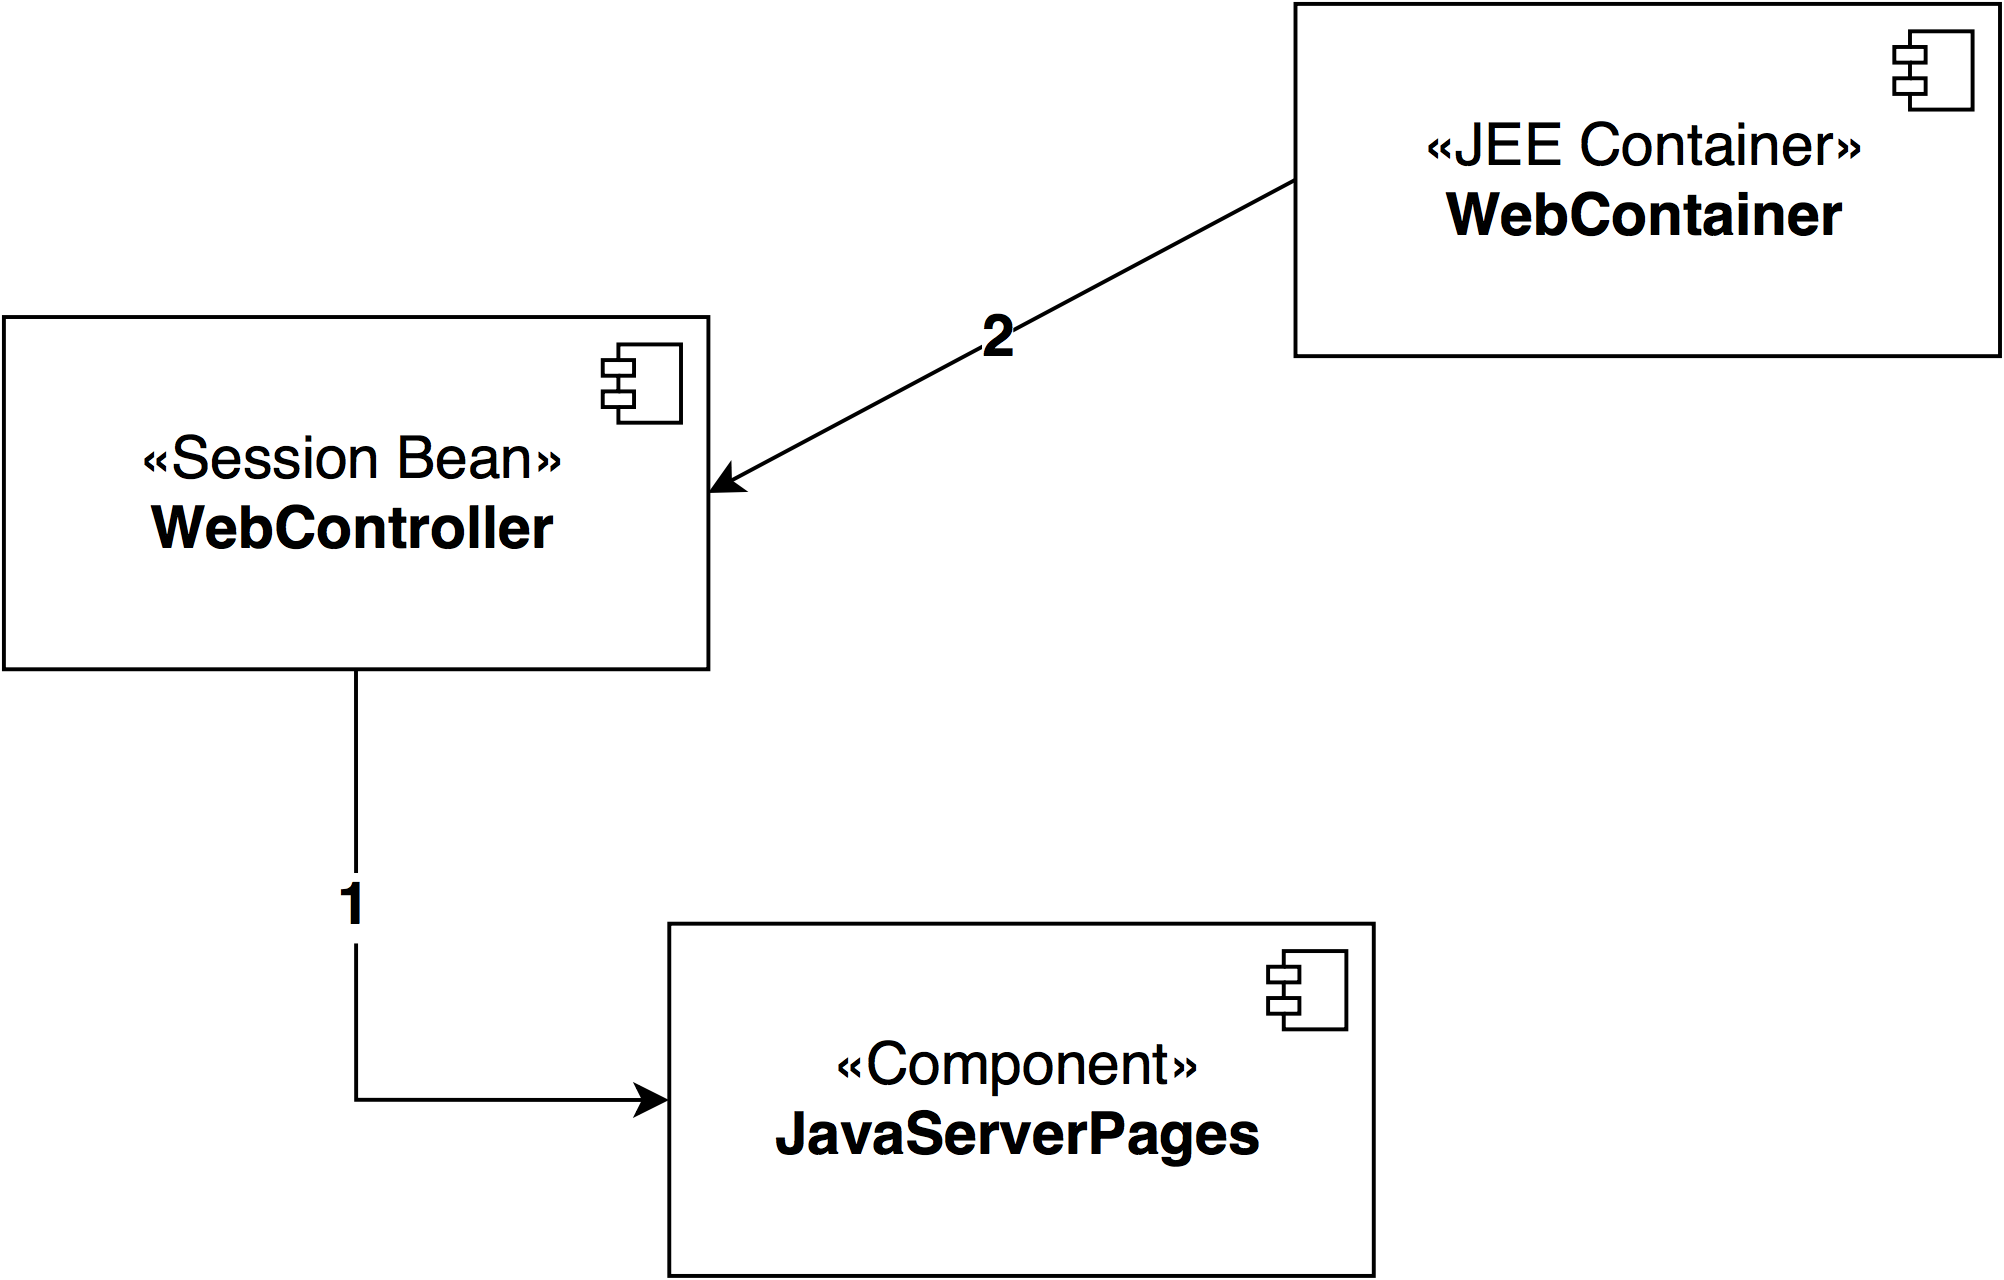
\includegraphics[width=0.3\textwidth]{./integration_strategy/diagrams/web.png}
\end{center}
\end{figure}

\begin{longtable}{p{0.05\textwidth} | p{0.3\textwidth} | p{0.3\textwidth} | p{0.3\textwidth}}
\hline
\textbf{N.} & \textbf{Subsystems} & \textbf{Component} & \textbf{Integrates with} \\
\hline
I01 & Database, App. Logic & (JEB) User & DBMS \\
\hline
I02 & Database, App. Logic & (JEB) Car & DBMS \\
\hline
I03 & Database, App. Logic & (JEB) Reservation & DBMS \\
\hline
I04 & Database, App. Logic & (JEB) Ride & DBMS \\
\hline
I05 & Database, App. Logic & (JEB) SafeArea & DBMS \\
\hline
I06 & Database, App. Logic & (JEB) PowerGridStation & DBMS \\
\hline
I07 & Database, App. Logic & (JEB) AlternativeChargesSitutation & DBMS \\
\hline
I08 & App. Logic, MaintenanceSystem & (EXT) MaintenanceSystemEndpoint & (SB) CarStatusManager \\
\hline
I09 & App. Logic & (SB) DiscountProvider & (JEB) AlternativeChargesSituation \\
\hline
I10 & App. Logic & (SB) CarStatusManager & (JEB) Car \\
\hline
I11 & App. Logic & (SB) ReservationManager & (SB) CarStatusManager \\
\hline
I12 & App. Logic & (SB) UserManager & (JEB) User, (SB) NotificationManager \\
\hline
I13 & App. Logic & (SB) PaymentGateway & (JEB) Payment,(SB) UserManager, (SB) NotificationManager, (SB) DiscountProvider, (EXT) \textit{[stub]} PaymentHandlerEndpoint \\
\hline
I14 & App. Logic & (SB) RideManager & (JEB) Ride, (SB) PaymentGateway, (SB) DiscountProvider, (SB) CarStatusManager \\
\hline
I15 & App. Logic & (SB) ReservationManager & (JEB) Car, (JEB) Reservation, (SB) CarStatusManager \\
\hline
I16 & App. Logic & (SB) SecurityAuthenticator & (JEB) User, (JEB) Reservation, (SB) RideManager \\
\hline
I17 & App. Logic & (SB) MapManager & (JEB) Car, (JEB) SafeArea, (JEB) PowerGridStation, (SB) SecurityAuthenticator \\
\hline
I18 & App. Logic & (EJB Container) UserManagementContainer & (SB) UserManager \\
\hline
I19 & App. Logic & (EJB Container) UtilitiesContainer & (SB) MapManager, (SB) NotificationManager \\
\hline
I20 & App. Logic & (EJB Container) ChargesManagementContainer & (SB) PaymentGateway, (SB) DiscountProvider \\
\hline
I21 & App. Logic & (EJB Container) RideManagementContainer & (SB) RideManager, (SB) ReservationManager, (SB) SecurityAuthenticator, (SB) CarStatusManager \\
\hline
I22 & App. Logic & ContainerController & (EJB Container) UserManagementContainer, (EJB Container) UtilitiesContainer, (EJB Container) ChargesManagementContainer, (EJB Container) RideManagementContainer \\
\hline
I23 & On-Board Client & ApplicationController & UIManager, GPSManager, ConnectivityUnit, DataProcessingUnit \\
\hline
I24 & Mobile Client & ApplicationController & UIManager, GPSManager \\
\hline
I25 & Web & WebController & JavaServerPages \\
\hline
\caption{Integration order of the system components. External components are marked with (EXT).}
\label{software_int}
\end{longtable}

\subsection{Subsystem Integration Sequence}
The integration sequence of the high-level subsystems is described in Figure \ref{h_level_subsys} and Table \ref{subsys_int}.

\begin{figure}[H]
\begin{center}
		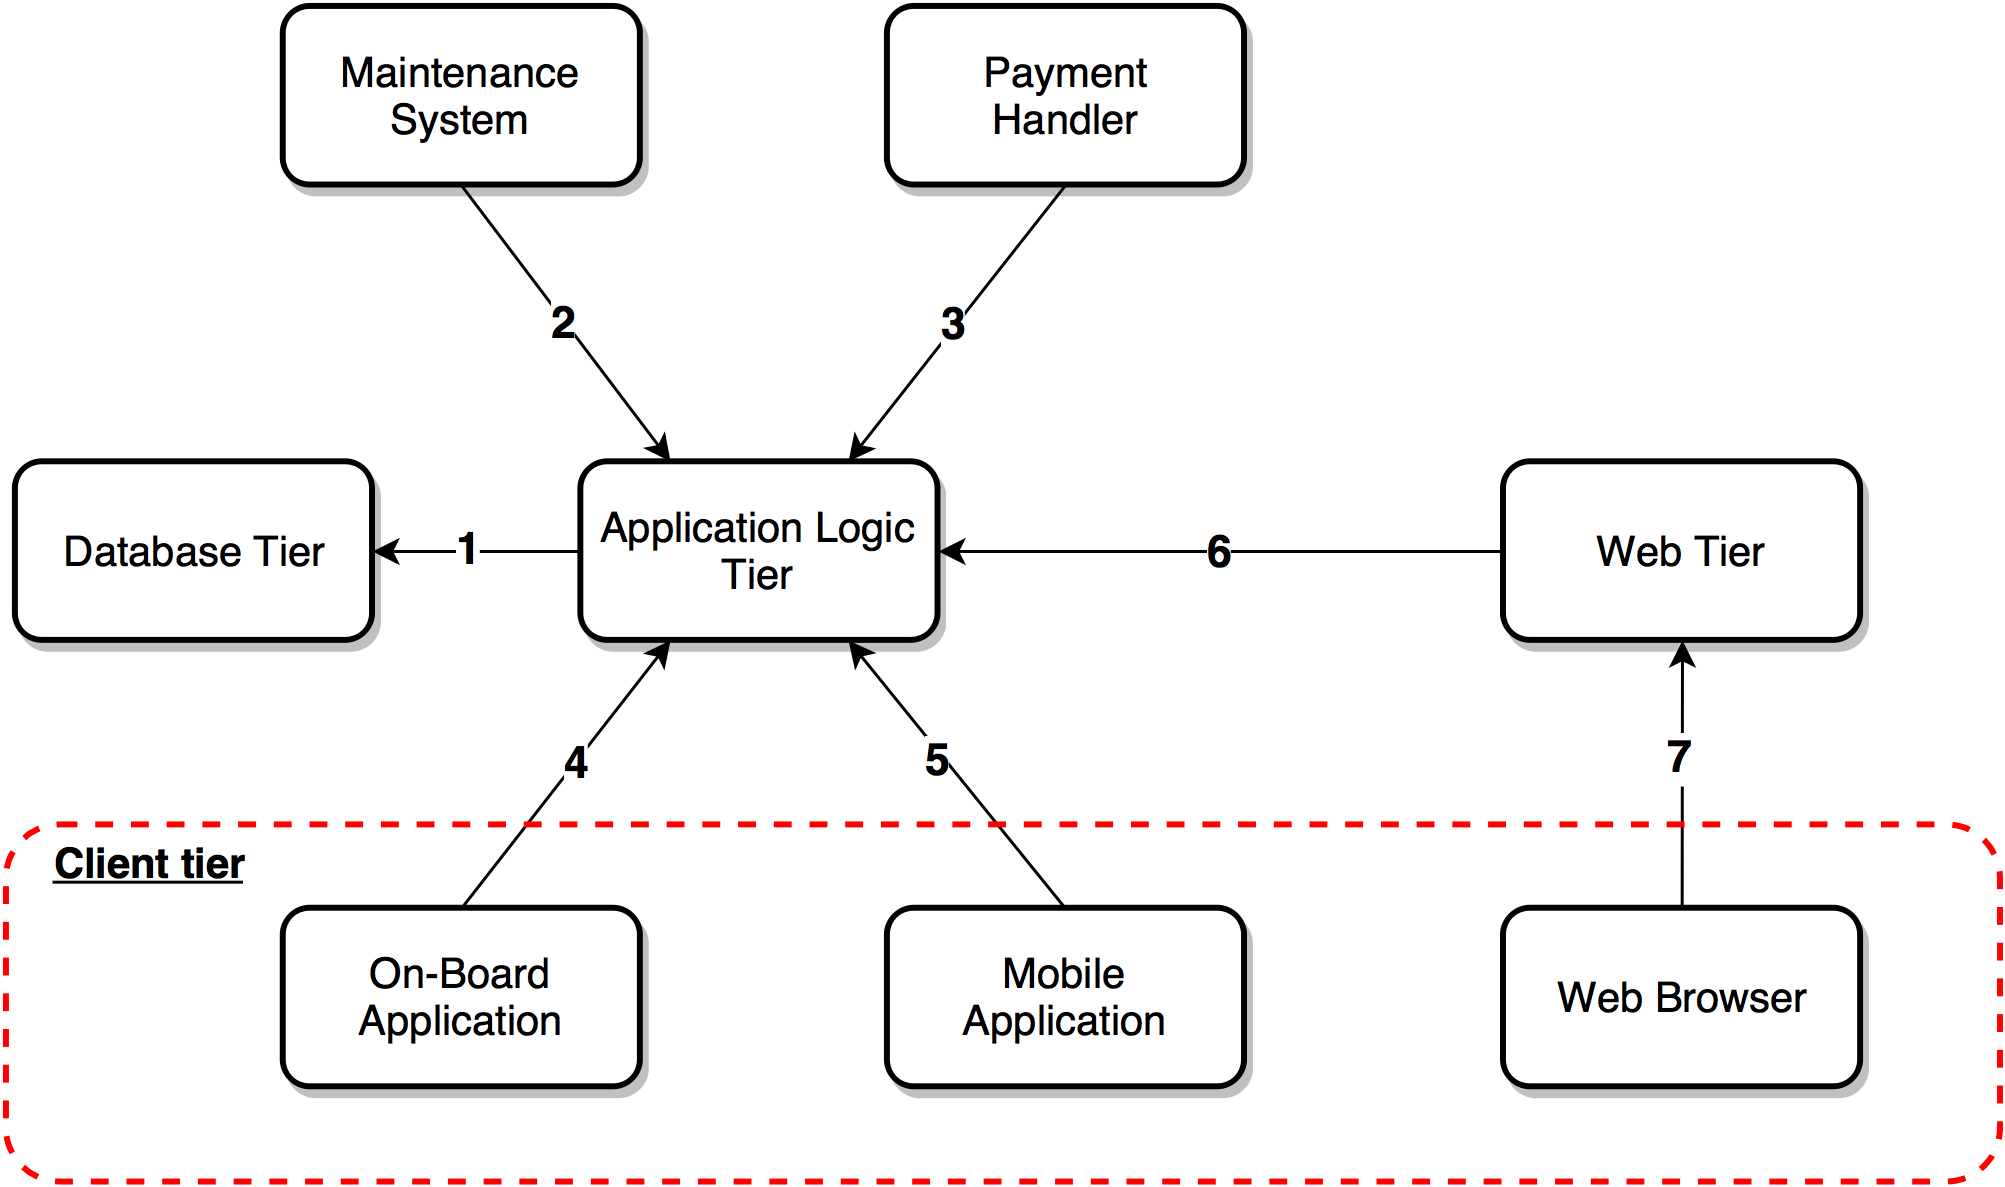
\includegraphics[width=\textwidth]{./integration_strategy/diagrams/h_level_subsys.png}
		\caption{Diagram representing the order of the subsystems integration.}
		\label{h_level_subsys}
\end{center}
\end{figure}

\begin{table}[H]
\begin{center}
\begin{tabular}{p{0.05\textwidth} | p{0.3\textwidth} | p{0.3\textwidth}}
\hline
\textbf{N.} & \textbf{Subsystem} & \textbf{Integrates with} \\
\hline
SI1 & Application Logic Tier & Database Tier \\
\hline
SI2 & On-Board Application & Application Logic Tier \\
\hline
SI3 & Mobile Application & Application Logic Tier \\
\hline
SI4 & Web Tier & Application Logic Tier \\
\hline
SI5 & Web Browser & Web Tier \\
\hline
\end{tabular}
\end{center}
\caption{Integration order of the subsystems described in Section \ref{elems_int}.}
\label{subsys_int}
\end{table}

Note that the base for the subsystem integration is the data tier, which is considered the most critical component; for the same reason, the application logic tier comes before all kinds of clients, since a working business logic is mandatory to have properly functioning clients. The choice of integrating the on-board application before other clients is due to the critical-module-first approach that has been chosen for this step of the integration process, since the on-board functionalities are meant to be core for the application itself. Lastly, the mobile application will be integrated first, since the integration of the web tier and browser client is heavier and more complex; moreover, this choice will allow the development team to have a working part of the system implementing a client-server structure even before having fully developed the web application.